\subsection{Affinity Diagram}\label{subsect:AffinityDiagram}
Following the collection of raw data from the survey, we applied the Affinity Diagram methodology to systematically organize facts, opinions, and insights. This collaborative UX mapping activity was executed through a structured 8-step process to synthesize the research findings before defining the User Personas.

\paragraph{Steps 1 \& 2: Data Collection and Sticky Notes Generation}
We began by extracting the most relevant qualitative and quantitative information from the 81 valid questionnaire responses. We translated these data points into virtual sticky notes using \textbf{Figma}. The notes included direct quotes, statistics, and recurring pain points. For instance, client-side notes highlighted phrases like \textit{"I use paper, pen, or phone notes to track my workouts"} or \textit{"Switching between multiple apps for workouts and diets is highly frustrating,"} while professional-side notes emphasized \textit{"WhatsApp and Excel are chaotic for managing multiple clients."}

\paragraph{Steps 3, 4 \& 5: Clustering, Labeling, and Combining}
Once the digital board was populated, we grouped the notes into clusters based on natural relationships and labeled them according to their core themes. By combining similar concepts, three overarching macro-themes emerged:
\begin{itemize}
    \item \textbf{The Burden of Digital Fragmentation:} a massive cluster formed around the inefficiency of current tracking methods. Sticky notes indicating the use of pen and paper, phone notes, and the simultaneous use of multiple apps were combined under this theme. The high frustration scores recorded in the survey strongly validated this label;
    \item \textbf{Inefficient B2C Communication:} this cluster grouped the professionals' administrative struggles (e.g., relying on generic messaging apps) with the clients' desire for a stronger, digital connection with their Personal Trainers. It highlighted the friction in exchanging feedback and updating diet/workout plans;
    \item \textbf{The "All-in-One" Demand:} a solution-oriented cluster aggregating the highly requested core features: unified workout tracking, integrated diet management, and digital facility access via QR code. 
\end{itemize}

\begin{figure}[H]
    \centering
    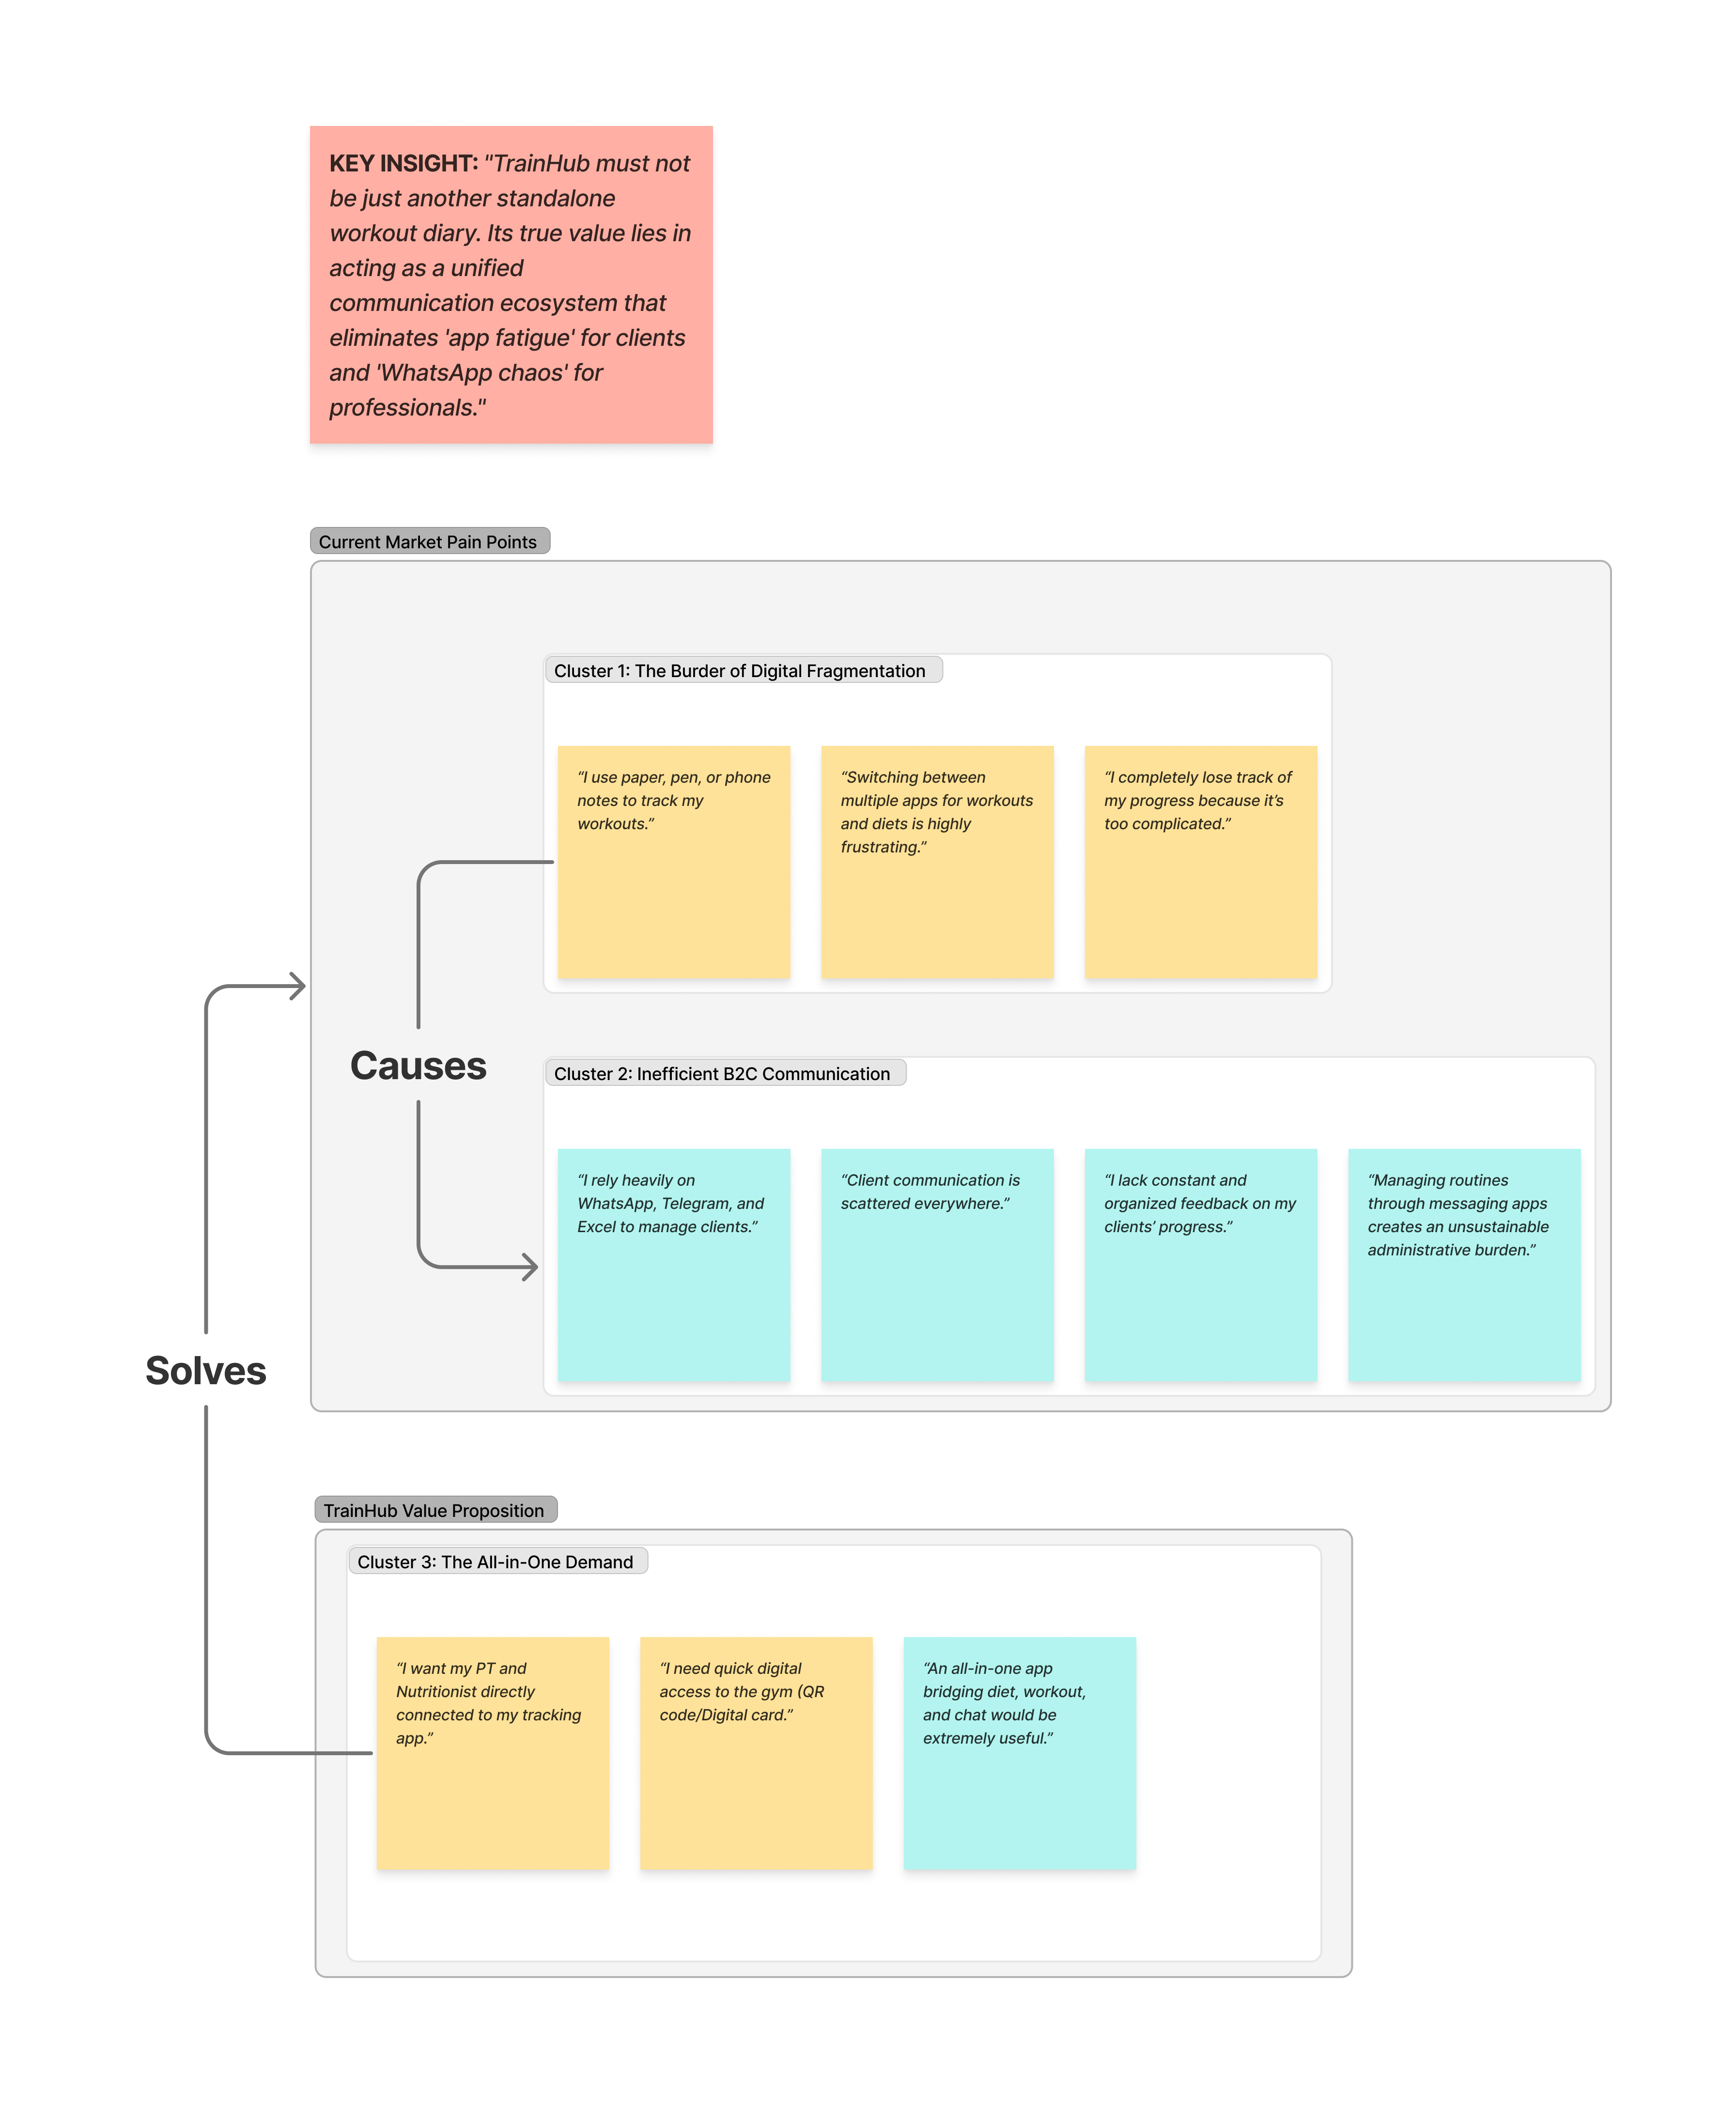
\includegraphics[width=0.9\textwidth]{3-UserResearch/img/AffinityDiagram/AffinityDiagram.jpg}
    \caption{Affinity Diagram board developed in Figma containing the clustered sticky notes.}
    \label{img:AffinityDiagramBoard}
\end{figure}

\paragraph{Step 6: Linking Dependencies}
After defining the macro-themes, we mapped the dependencies between the clusters. The structural link became evident: the \textit{Burden of Digital Fragmentation} (cause) directly forces professionals to resort to \textit{Inefficient B2C Communication} (effect), leading to poor tracking and frustrated users. The \textit{"All-in-One" Demand} acts as the structural bridge capable of resolving these dependencies by unifying the ecosystem.

\paragraph{Steps 7 \& 8: Interpretation and Documentation}
The final interpretation of this affinity mapping exercise provided a clear design directive. The diagram confirmed that TrainHub's core value does not simply lie in offering a digital workout diary, but rather in acting as a centralized communication hub that eliminates the "app fatigue". Documenting this process allowed us to confidently transition from raw, scattered survey data to well-defined, evidence-based user profiles. The insights finalized in this section directly shaped the goals and frustrations of the User Personas presented in the following paragraphs.
